%%%==============================================================================
% WinEdt pragmas
% !Mode:: "TeX:EN"
% Default Compile engines:
% !TEX program = pdflatex
% !PDFTeXify ext =  --enable-etex  --restrict-write18
% !PDFLaTeX ext  =  --enable-etex  --restrict-write18
% !BIB program = biber
%%%==============================================================================
%% Copyright 2022-present by Alceu Frigeri
%%
%% Document (sample) file using the class ufrgscca
%%
%% This file was adapted from:
%% Meta-monografia de exemplo genérico de uso da classe delaetex.cls
%% Copyright (C) 2004..2016 Walter Fetter Lages <fetter@ece.ufrgs.br>
%%
%%%==============================================================================
%\documentclass[repeatfields,openright,overleaf,nomicrotype]{ufrgscca}
\documentclass[repeatfields,xlists,xpacks,oneside]{ufrgscca}


\addbibresource{modeloTCC.bib}


%%%%%%%%%%%%%%%%%%%%%%
%%%%%%%%%%%%%%%%%%%%%%
%%
%% TCC Class options
%%
%% english   => paper/report in english
%%     \documentclass[english]{tcc}
%%
%% repeatfields => (abnt) references with same authors have their names repeated.
%%												otherwise only the first reference of them will be printed.
%%     \documentclass[repeatfields]{tcc}
%%
%% openright => force the start of a chapter at odd pages.
%%     \documentclass[openright]{tcc}
%%
%% oneside => single side document
%%     \documentclass[oneside]{tcc}
%%
%% NOTE : openright, oneside :: IF you are going to print the doc, single sided, the best is to just use
%%                              the [oneside] option.
%%                              IF you are going to print the doc, double sided, the best is to just use the
%%                              the [openright] option.
%%
%% relnum => figures/tables counters are reset with each chapter.
%%     \documentclass[relnum]{tcc}
%%
%% showframe => (for drafts only) auxiliary visual guide to page frame.
%%     \documentclass[showframe]{tcc}
%%
%% showlabels =>  (for drafts only) prints labes/citeref strings on the side bar.
%%     \documentclass[showlabels]{tcc}
%%
%%
%%%%%%%%%%%%%%%%%%%%%%
%%%%%%%%%%%%%%%%%%%%%%

%
% inicio do documento
%

\begin{document}



%%%%%%%%%%%%%%%%%%%%%%
%%%%%%%%%%%%%%%%%%%%%%
%%
%% \MakeCoverPages produz as páginas iniciais
%% as opções são
%%
%% tccI => para TCC-I
%% tccII => para TCC-II
%% internship => para Estágio Obrigatório
%% internship-opt => para Estágio Não Obrigatório
%% class-report => para relatórios/trabalhos de uma disciplina
%%
%%%%%%%%%%%%%%%%%%%%%%
%%%%%%%%%%%%%%%%%%%%%%

%\MakeCoverPages{tccI}
\MakeCoverPages{tccII}

% dedicatoria é opcional
%\nonum\chapter{Dedicatória} %vai ter uma entrada no sumário
\notoc\chapter{Dedicatória} %não vai aparecer no sumário

Dedico este trabalho aos meus pais, em especial pela dedicação e apoio em
todos os momentos difíceis.

% agradecimentos são opcionais
%\nonum\chapter{Agradecimentos}
\notoc\chapter{Agradecimentos}

\`{A} Universidade Federal do Rio Grande do Sul, UFRGS, pela
oportunidade de realização de estudos.

Aos colegas de curso pelo seu auxílio nas tarefas desenvolvidas durante o
curso e apoio na revisão deste trabalho.

Agradeço ao \LaTeX\ por não ter vírus de macro\ldots


% palavras-chave
% iniciar todas com letras minúsculas, exceto no caso de abreviaturas
%
\mainkeywords{Engenharia Elétrica}
\mainkeywords{Processamento de Sinais}
\mainkeywords{Automação e Controle}
\mainkeywords{Eletrônica e Instrumentação}


% resumo no idioma do documento
\begin{mainabstract}

Este documento foi criado com o objetivo de auxiliar aos alunos
de graduação
da Universidade Federal do Rio Grande do Sul (UFRGS) no desenvolvimento dos
volumes finais de seus trabalhos de conclus\~{a}o de curso. O presente
documento serve, ao mesmo tempo, como modelo do formato de apresentação
oficial do TCC-CCA, bem como de roteiro para as etapas de elaboração do texto
técnico que o compõe. Os modelos e formatações aqui contidos são baseados em
normas da Associação Brasileira de Normas Técnicas (ABNT), em especial a
NBR-14724~\cite{ABNT:NBR-14724-2011}, que descreve o procedimento de elaboração e
apresentação de trabalhos acadêmicos (dissertações, teses, monografias,
entre outros).

\end{mainabstract}

% resumo no outro idioma
% como parametro devem ser passadas as palavras-chave
% no outro idioma, separadas por vírgulas

\otherkeywords{Electrical Engineering}
\otherkeywords{Signal Processing}
\otherkeywords{Automation and Control}
\otherkeywords{Electronic and Instrumentation}

%%
%% No caso do documento ser em ingles, usar
%%  \begin{otherabstract}[brazilian]
%%
\begin{otherabstract}
This document aims to support undergraduated students  of Universidade Federal do Rio
Grande do Sul (UFRGS) in the development of their diplom project relatory.
This document serves concomitantly as a model of the official TCC-CCA
presentation layout as well as a guide throughout technical text composition
steps. The model and format held here are based in norms of the Associação
Brasileira de Normas Técnicas (ABNT), mainly in
NBR-14724~\cite{ABNT:NBR-14724-2011} which defines guidelines of design and
presentation of academic documents.
\end{otherabstract}


% sumario
\setcounter{tocdepth}{3}

% lista de ilustrações
\listoffigures

% lista de tabelas
\listoftables

% lista de listagens (código fonte)
\listofcodelist %% doesn't work on overleaf

% lista de abreviaturas e siglas
% o parametro deve ser a abreviatura mais longa
\begin{listofabbrv}{PPGEE}
	\item[ABNT] Associação Brasileira de Normas Técnicas
	\item[GCAR] Grupo de Controle, Automação e Robótica
	\item[PPGEE] Programa de Pós-Graduação em Engenharia Elétrica
	\item[CCA] Curso de Eng. em Controle e Automação
\end{listofabbrv}

% lista de símbolos é opcional
\begin{listofsymbols}{$\alpha\beta\pi\omega$}
       \item[$\sum$] Somatório
       \item[$\alpha\beta\pi\omega$] Fator de inconstância do resultado
\end{listofsymbols}


\tableofcontents


% AQUI COMEÇA O TEXTO PROPRIAMENTE DITO

% introducao
\chapter{Introdução}

O trabalho de conclusão de curso, TCC,  representa o resultado
final dos trabalhos desempenhados pelo aluno durante o seu período de graduação na UFRGS.

Ao iniciar as etapas propriamente relacionadas com o TCC,
o aluno deve realizar uma pormenorizada pesquisa bibliográfica, procurando
todos relevantes trabalhos relacionados com o tema proposto e definindo a
abordagem a ser utilizada. Já nesta parte é importante preocupar-se com a
documentação técnica destes trabalhos como forma de contextualização e
justificativa do trabalho  alvo.

O volume final deve conter uma apresentação clara e cientificamente embasada
da(s) técnica(s) utilizada(s), descrição do(s) modelo(s) proposto(s) ou
utilizado(s), detalhamento das experiências práticas e apresentação das
conclusões finais levantadas pelo autor.

Deve-se destacar que uma TCC é,
acima de tudo, um documento científico e como tal precisa ser considerada
durante sua elaboração. O documento deve ser escrito, com vocabulário
técnico adequado, de forma a gerar uma descrição clara e objetiva dos
trabalhos desenvolvidos pelo autor.

Como forma de auxílio aos alunos durante a escrita de seus trabalhos de conclusão de curso, bem como de padronização dos documentos publicados, este modelo foi criado. Alguns itens são sugestões outros são
obrigatórios, tais como: capa, folha de rosto, folha de aprovação, resumo,
abastract, sumário, lista de figuras, lista de tabelas, lista e abreviaturas
e referências bibliográficas. Tomando-o como base tornam-se facilitadas as
etapas de estruturação e formatação do documento a ser elaborado pelo aluno.

O capítulo~\ref{revisao} deste documento serve de modelo para a seção de
revisão de literatura. O capítulo~\ref{partes} apresenta detalhadamente
as demais partes (obrigatórias ou não) constituintes do documento final. O
modelo de formatação do documento é apresentado no capítulo~\ref{formas},
enquanto que o capítulo~\ref{conclusao} serve de base para a seção de
conclusões.

\chapter{Revisão da Literatura}
\label{revisao}

Para a elaboração deste documento foram revisadas as normas vigentes no país
para projeto e diagramação de textos técnicos para o meio acadêmico. A fim
de melhor entender a abrangência de cada norma uma descrição resumida desta
é apresentada a seguir.

A norma brasileira NBR-14724~\cite{ABNT:NBR-14724-2011} descreve o modelo de
apresentação de trabalhos acadêmicos reconhecido nacionalmente.

A norma NBR-6024~\cite{ABNT:NBR-6024-2003}  apresenta os procedimentos para
elaboração de numeração progressiva das seções de um documento.

A norma  NBR-6023~\cite{ABNT:NBR-6023-2002} apresenta o procedimento padrão
para elaboração de referências.

A norma NBR-6027~\cite{ABNT:NBR-6027-2003} apresenta o modelo de construção do sumário.

A norma NBR-6028~\cite{ABNT:NBR-6028-2003} apresenta o modelo de construção do resumo.

A norma NBR-6034~\cite{ABNT:NBR-6034-2004} apresenta os procedimentos para construção de um índice.

A norma NBR-10520~\cite{ABNT:NBR-10520-2002} descreve sobre as
formas de apresentação de citações em documentos.


Note que tabelas devem ser construídas seguindo o modelo desenvolvido pelo IBGE \cite{IBGE:tabular-1993}.
%A norma NBR-12225~\cite{ABNT:NBR-12225} apresenta o modelo de construão de lombada de volume.


A seção de revisão de literatura (ou estado da arte) do aluno deve ser
elaborada de forma similar ao texto aqui apresentado, citando todos os
trabalhos relevantes publicados na área de abrangência de sua proposta e
apresentando uma descrição resumida de seus conteúdos.

\chapter{As Partes de um TCC}
\label{partes}


Segundo norma NBR 14724~\cite{ABNT:NBR-14724-2011},
de uma monografia / trabalho científico devem constar as seguintes partes principais ou
elementos:

\begin{tabular}{rrl}
\ldelim\{{2}{*}[Parte Externa\hfill] & & Capa (obrigatório) \\
                                  & & Lombada (opcional) \\ \\
\ldelim\{{23}{*}[Parte Interna\hfill] & \ldelim\{{13}{*}[Elementos pré-textuais] & Folha de rosto (obrigatório)\\
 & & Errata (opcional)\\
 & & Folha de aprovação (obrigatório)\\
 & & Dedicatória (opcional)\\
 & & Agradecimentos (opcional) \\
 & & Epígrafe (opcional) \\
 & & Resumo na língua vernácula (obrigatório)\\
 & & Resumo em língua estrangeira (obrigatório)\\
 & & Lista de ilustrações (opcional)\\
 & & Lista de tabelas (opcional)\\
 & & Lista de abreviaturas e siglas (opcional)\\
 & & Lista de símbolos (opcional)\\
 & & Sumário (obrigatório)\\ \\
                                  & \ldelim\{{3}{*}[Elementos textuais] & Introdução\\
																	& & Desenvolvimento\\
																	& & Conclusão\\ \\
																	& \ldelim\{{5}{*}[Elementos pós-textuais] & Referências (obrigatório)\\
																	& & Glossário (opcional)\\
																	& & Apêndice (opcional)\\
																	& & Anexo (opcional)\\
																	& & Índice (opcional)
\end{tabular}


\section{Parte Externa}

\subsection{Capa}

A capa deve conter na sequência apresentada os seguintes elementos:

\begin{enumerate}[tcc,alpha)]
\item descrição da unidade (Universidade, Escola e Departamento);
\item nome do autor;
\item título;
\item subtítulo (se houver);
\item número de volume (se houver mais de um volume);
\item local onde foi apresentado o trabalho;
\item ano de depósito (ou entrega do trabalho).
\end{enumerate}

Note que a capa não faz parte do texto, não sendo contabilizada para o número de páginas do texto.

\section{Parte Interna}

\subsection{Elementos Pré-textuais}

Estes elementos antecedem o texto propriamente dito e contêm informações que
ajudam na identificação e uso do trabalho.

\begin{equation}
    R_{1,2}=\frac{-b\pm\sqrt{b^2-4ac}}{2a}
\end{equation}



Cada um destes itens deve ocupar uma ou mais páginas separadas e a ordenação
(paginação ou numeração), embora não apareça impressa, começa na página 1
(folha de rosto).


\subsubsection{Folha de Rosto}

A folha de rosto deve conter:

\begin{enumerate}[tcc,alpha)]
\item nome do autor;
\item título do trabalho (e subtítulo, quando for necessário);
\item número do volume (se caracterizar parte de uma obra);
\item natureza (tese, dissertação, etc\ldots) e objetivo (aprovação, grau pretendido e outros);
\item nome do orientador (e co-orientador, se houver);
\item local;
\item ano do depósito.
\end{enumerate}

\subsubsection{Folha de Aprovação}

A folha de aprovação, que discrimina a banca examinadora do trabalho, deve
conter na ordem os seguintes itens:

\begin{enumerate}[tcc,alpha)]
\item autor (nome completo no topo da página);
\item título do trabalho (e subtítulo, se houver, seguido por dois pontos ":");
\item local e data da apresentação;
\item nome e assinatura do orientador;
\item nome e instituição dos membros componentes da banca;
\item nome e assinatura do coordenador de curso.
\end{enumerate}

\subsubsection{Dedicatória}

Este item opcional permite que se faça menção explícita e direta de
pessoa(s) ou entidade(s) de grande importância para o autor, de forma a
receber citação especial nesta folha.

\subsubsection{Agradecimentos}

A folha de agradecimentos, também opcional, serve para o autor, que deseje
expressar sua consideração a parentes, colegas, amigos, professores e/ou
entidades, que participaram no desenvolvimento de seu trabalho, de forma a
destacá-los também no corpo do documento.

\subsubsection{Epígrafe}

A epígrafe, quando houver, permite que o autor apresente uma citação seguida
de indicação de autoria, relacionada com a matéria tratada no corpo do
trabalho. Este elemento, entretanto, não é recomendado por este Programa.

\subsubsection{Resumo}

O resumo deve ser uma apresentação concisa e objetiva, em um único
parágrafo, que apresente o conteúdo e conclusões da dissertação (ou tese),
estando limitado pelo uso máximo de 500 palavras. Ao final deste, devem-se
seguir as Palavras-chaves que descrevem e detalham mais explicitamente o
escopo do trabalho.

\subsubsection{Abstract}

Uma transcrição do resumo para o inglês (devidamente revisada) deve também
ser incluída, denominando-se esta de Abstract. Este também deve ser seguido
da versão em inglês das palavras-chaves, denominada de Keywords. Além do
Abstract, quando existe interesse por parte do pesquisador e orientador
pode-se acrescentar mais uma versão do resumo em outra língua estrangeira
(tal como alemão, francês, etc.), devidamente aprovada por professor com
fluência na língua em questão.

\subsubsection{Sumário}

O sumário consiste na enumeração das principais divisões do trabalhos, feita
na mesma ordem em que se sucedem no corpo do texto, seguida da respectiva
paginação. O Sumário deve ser elaborado usando-se os mesmos formatos
(fontes, tamanho, etc) usados nos separadores de seção e subseção,
considerando-se até o terceiro nível de divisões.

\subsubsection{Lista de Ilustrações}

A lista de ilustrações é elaborada de acordo com a ordem das figuras
encontradas no texto, indicando cada legenda de ilustração acompanhada do
respectivo número de página. Devem ser contínuas em todo o texto,
independente do capítulo.

\subsubsection{Outras listas, a semelhança de ilustrações}

É possível diferenciar-se, caso necessário, tipos de figuras, e.g., "Desenho", "Esquema", "Fluxograma", "Fotografia", etc. os procedimentos são os mesmos.
Cada lista deve ser  elaborada de acordo com a ordem encontrada no texto,
indicando a legenda  acompanhada do
respectivo número de página. A numeração deve ser contínua em todo o texto,
independente do capítulo.


\subsubsection{Lista de Tabelas}

A lista de tabelas é elaborada segundo a ordem de ocorrência de tabelas no
texto, apresentando cada descrição de tabela acompanhada do respectivo
número de página. Assim como para a lista de ilustrações, devem também ser
contínuas em todo o texto, independente do capítulo.


\subsubsection{Lista de Abreviaturas}

Constitui-se de uma relação alfabética das abreviaturas e siglas encontradas
no texto, seguidas das palavras ou expressões que representam, grafadas por
extenso.

\subsubsection{Lista de Símbolos}

A Lista de Símbolos, quando existir, deve ser elaborada de acordo  com a
ordem apresentada no texto, seguida pelo devido significado.

\subsection{Elementos Textuais}

Os elementos textuais compõem a parte do documento onde o trabalho
desenvolvido é propriamente descrito.

O corpo do texto é dividido em diversos capítulos numerados sequencialmente
por algarismos arábicos.

\subsection{Elementos de Pós-Textuais}

Os elementos de complementação ou elementos pós-textuais acrescem
informações relevantes ao trabalho técnico desenvolvido. Podem apresentar as
seguintes partes:

\begin{enumerate}[tcc,alpha)]
\item referências (obrigatório);
\item apêndices (opcional);
\item anexos (opcional);
\item glossário (opcional).
\end{enumerate}

O capítulo referências apresenta uma relação padronizada dos artigos e
trabalhos utilizados pelo autor da dissertação (ou tese).

Nos capítulos apêndices (textos produzidos pelo autor) e anexos (documentos
de terceiros) são colocadas citações muito longas para o texto, deduções
auxiliares, listagens de programas, ilustrações e estatísticas
complementares para o trabalho.

\subsubsection{Referências}
O formato padronizado de referências a ser seguido baseia-se na norma da ABNT
NBR-6023~\cite{ABNT:NBR-6023-2002}. São considerados
elementos essenciais para toda e qualquer referência, nome(s) do(s)
autor(es), título do documento, local e data de publicação. Detalhes específicos podem ser vistos em \autonameref{sec:referencias}.


\subsubsection{Apêndices}

Nos apêndices aparecem textos ou documentos {\bf elaborados pelo autor}  a
fim de complementar sua argumentação sem prejuízo do trabalho. Eles sempre
deverão estar antes dos anexos. Se o documento incluir mais de um texto de
Apêndice, os indicativos de apêndices devem ser identificados por letras
maiúsculas seguidos pelos respectivos títulos. Exemplo:\\

\begin{quote}APÊNDICE A  - OUTROS EDITORES\\\end{quote}

\subsubsection{Anexos}

Já os anexos serão textos, trabalhos e materiais que {\bf não foram
elaborados pelo autor}, mas que servem de comprovação, fundamentação ou
ilustração dos argumentos contidos no texto. Os anexos, assim como os
apêndices, se forem mais de um, devem ser identificados por letras
maiúsculas e os respectivos títulos:\\

\begin{quote}ANEXO A - ORIENTAÇÃO DE ESTILO PARA APRESENTAÇÃO DE TRABALHOS - UNIVERSIDADE FEDERAL DO PARANÁ\\\end{quote}

\subsubsection{Glossário}

O glossário consiste de uma lista em ordem alfabética de palavras ou
expressões técnicas de uso restrito ou sentido obscuro, utilizadas no texto,
e acompanhadas das respectivas definições. Um glossário é opcional.

\chapter{Formas de Apresentação de um Trabalho de Conclusão de Curso}
\label{formas}

\section{Formato}

O trabalhor deverá ser impresso somente em uma face de folha de papel
branco no formato A4 (210x297 mm), no tamanho 12 a 20 cm para títulos de
seção e subseção (incluindo resumo, abstract, sumário, lista de figuras,
lista de tabelas, lista de abreviaturas e referências), e no tamanho 10 a 12
cm para textos.

As margens deverão medir de 2 a 4 cm.

Os textos do resumo e abstract deverão ser digitados em um único parágrafo
sem inserção de tabuladores (tabs).

O espaçamento entre as linhas a ser usado poderá ser simples ou duplo.

As notas de rodapé deverão ser digitadas dentro das margens
propostas\footnote{Textos de rodapé são identificados com numeração
contínua, reiniciando a cada capítulo da obra}, separadas do texto por um
espaço simples a partir da margem esquerda.

\section{Indicativos de Seção}

Os títulos de cada seção primária (capítulo) devem iniciar em folha
distinta.

Os títulos das seções e subseções devem apresentar numeração progressiva,
com separação entre níveis (separador presente entre números) utilizando
carater ponto ". ".

\section{Paginação}

A partir da folha de rosto as páginas são contadas, apresentando numeração
impressa entretanto só a partir da primeira folha da parte textual, em
algarismos arábicos no canto superior direito, distanciado de 2 cm das
bordas superior e direita. No caso de mais de um volume, deve-se usar uma
única sequência. Apêndices e anexos são numerados de maneira contínua como
segmentos do texto principal.

\section{Citações}

As citações de referências devem ser feitas em letras maíusculas, entre
parênteses, especificando as informações principais de sobrenome do autor e
ano da publicação.\\

Exemplo: Segundo~\cite{Brito:IEE-1994} esta técnica propicia maior
resolução\ldots\\

Sistemas modernos de comunicação sem fio~\cite{Bilstrup:FCS-239}\ldots\\

Uma forma alternativa de fazer uma citação é indicando o nome do autor no
texto, como pode ser visto no exemplo a seguir, desde que o autor seja
claramente discriminado no capítulo de referências. Não é entretanto um
formato recomendado pelo Programa.\\

Exemplos: Segundo~\textcite{Brito:IEE-1994} esta técnica propicia maior
resolução\ldots\\

Quando houver coincidência de autores com mesmo sobrenome e data deve-se
acrescentar as iniciais de seus prenomes. As citações de diferentes
documentos de mesmo autor, publicados em um mesmo ano são distinguidas, pelo
acréscimo de letras minúsculas após a data sem espaço, as quais devem também
ser acrescidas nas referências do documento.\\

Exemplos: Conforme \cite{Pereira:OORT1999-133} ou \cite{Pereira:OORT1999-155} e
\cite{Pereira:RTP1999-9} percebe-se \ldots\\

As citações de diversos documentos distintos que necessitem ser feitas no
mesmo ponto do texto, devem ser separadas por ponto-e-vírgula. Recomenda-se
que as mesmas sejam indicadas dentro de parênteses como no exemplo a
seguir.\\

Exemplo: Outros sistemas de
monitoração~\cite{Baturone:DCIS1996-231,Cota:TIM-49-2}\ldots\\

\section{Abreviaturas e Siglas}

Quando aparecerem pela primeira vez no texto, deve-se colocar seu nome por
extenso, acrescentando-se a abreviatura ou sigla entre parênteses.

Exemplo:   Grupo de Controle, Automação e Robótica (GCAR)

\section{Equações e Fórmulas}

Equações e fórmulas dentro de parágrafos permitem o uso de entrelinhas
maiores de forma a comportar seus elementos sem corte, tais como expoentes,
índices, etc.

Quando destacadas do parágrafo são centralizadas e, se necessário, devem ser
numeradas de forma consecutiva, com número indicado no canto direito.

\begin{equation}
R_{1,2}=\frac{-b\pm\sqrt{b^2-4ac}}{2a}
\end{equation}

Quando fragmentadas em mais de uma linha, por falta de espaço, devem ser
interrompidas antes do sinal de igualdade ou depois dos sinais de adição,
subtração, multiplicação e divisão. Exemplo:

\begin{eqnarray}
R^k &=& B^k \sum_{i=1}^{n-1}{\left(H_{tc}^{k_i}+I_{tc}^k\right)}+H_m^k+(m-1)\lambda \nonumber\\
&=& B^k \sum_{i=1}^{n-1}{\left(nh\pi_{tc}^kCh_{max}^k+I_{tc}^k\right)}+nh\pi_m^k+(m-1)\lambda
\end{eqnarray}


\section{Ilustrações}

A identificação de ilustrações aparece sempre na parte superior precedida da
palavra "Figura"\ seguida do número em ordem de ocorrência no texto, em
algarismos arábicos, e respectivo título e/ou legenda explicativa,
apresentados de forma breve e clara. As ilustrações devem ser inseridas o
mais próximo possível do trecho a que se referem.

A seguir são apresentados alguns exemplos de figuras.

\begin{figure}[htbp]
{
  \centering
  \caption{Ecocardiograma do corte "quatro cavidades"\ de um paciente normal.}
  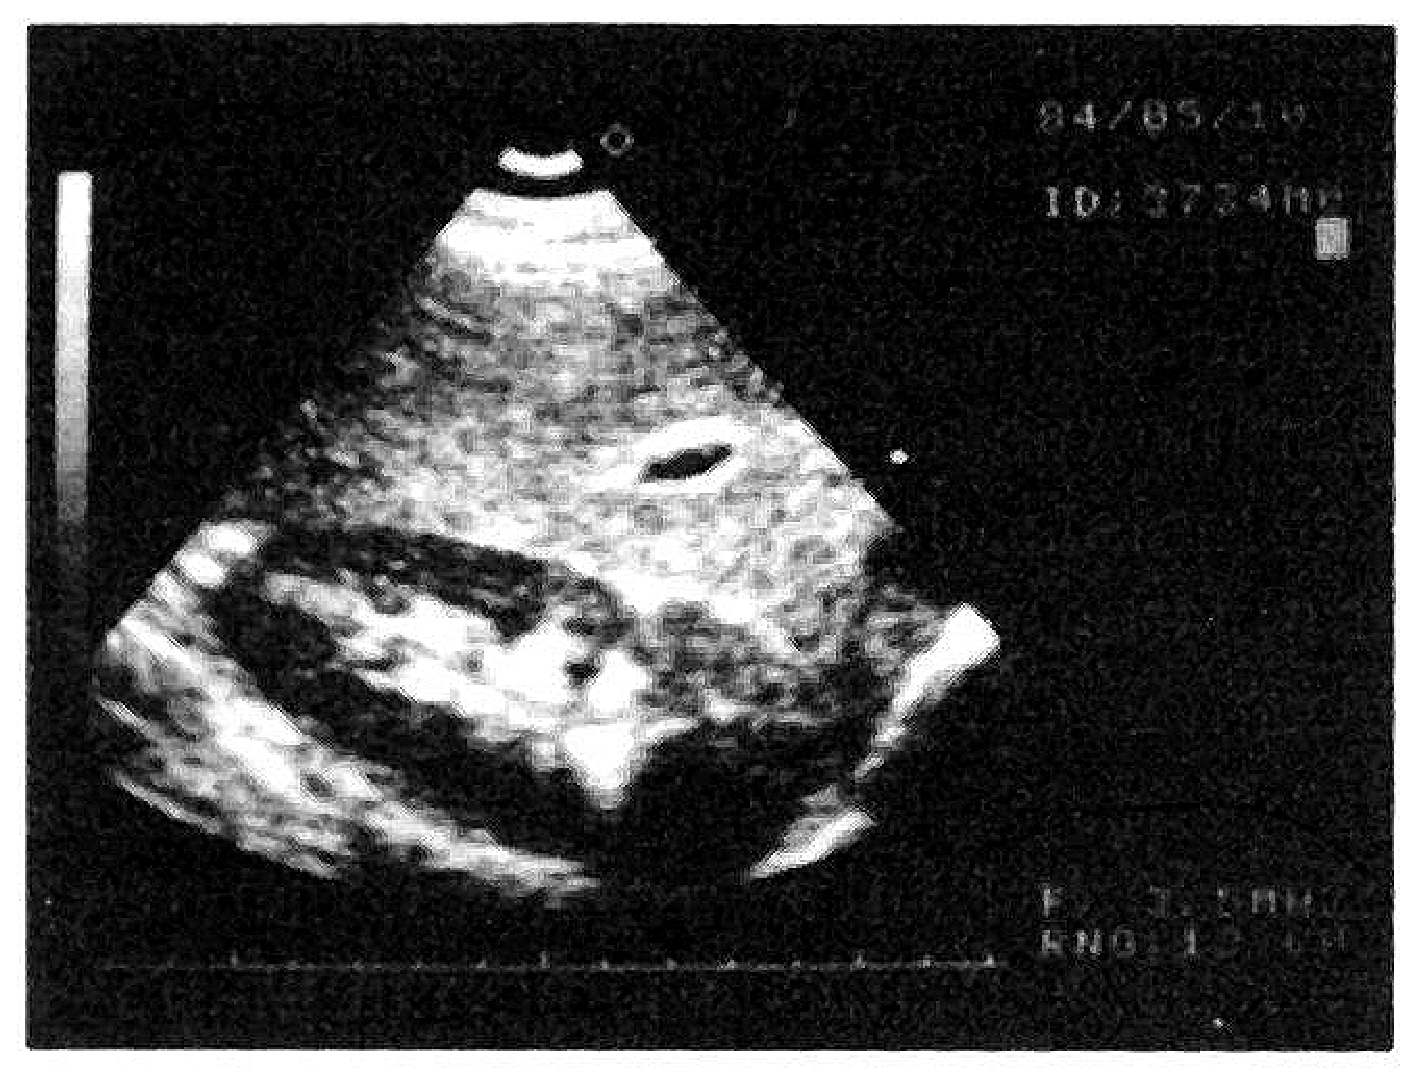
\includegraphics[width=0.33\textwidth]{eco}\\
}
{\sourcecitation{\textcite{Baturone:DCIS1996-231,Cota:TIM-49-2}}}
\note{Em alguns casos pode ser necessário/interessante adicionar um texto explicativo junto à ilustração. Nestes casos o mesmo deve ser adicionado abaixo da ilustração, após a citação da fonte.}
\end{figure}

\begin{figure}[htbp]
{
  \centering
  \caption[Simulação de motor síncrono monofásico.]{Simulação de motor síncrono monofásico nas condições específicas conforme texto (note que é possível ter-se um título longo junto a ilustração e um título curto para a lista de figuras)}
  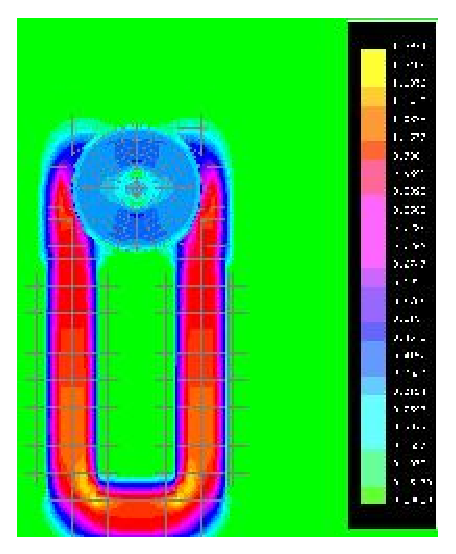
\includegraphics[width=0.2\textwidth]{motor}\\
}
{\sourcecitation{\textcite{Garg:SMA-2000}}}
\end{figure}


\subsection{Circuitos, listagens  e outros tipos de ilustrações}

Circuitos, bloco diagramas, listagens de código fonte são, em princípio, apenas ilustrações, e como tal são tratados. Entretanto, caso o documento apresente um grande número de circuitos, pode-se diferenciar os mesmos, criando-se uma "lista de circuitos" (opcional, como descrito a seguir).

\begin{figure}[htbp]
{
  \centering
  \caption{Amplificador de dois estágios hibrído.}
\tikzset{blockdef/.style={%
%	{Straight Barb[harpoon, reversed, right, length=0.2cm]}-{Straight Barb[harpoon, reversed, left, length=0.2cm]},blue% DAMMIT BROKEN OVERLEAF
	}
}
 \def\killdepth#1{{\raisebox{0pt}[\height][0pt]{#1}}}
 \def\coord(#1){coordinate(#1)}
 \def\coord(#1){node[circle, red, draw, inner sep=1pt,pin={[red, overlay, inner sep=0.5 pt, font=\tiny, pin distance=0.1cm, pin edge={red, overlay,}]45:#1}](#1){}}
\begin{center}
\resizebox{0.65\textwidth}{!}{
\begin{circuitikz}[american, scale=0.8]
% \ctikzset{resistors/scale=0.7, capacitors/scale=0.6} % DAMMIT BROKEN OVERLEAF
 \draw (0,0) node[nmos,](Q1){\killdepth{Q1}};
 \draw (Q1.S) to[R, l^=$R_S$] ++(0,-3) node[vee](VEE){$V_{EE}=\SI {-10}{V}$}; %define VEE level
 \draw (Q1.S) to[short] ++(2,0) to[C=$C_1$] ++(0,-1.5) node[ground](GND){};
 \draw (Q1.G) to[short] ++(-1,0) \coord (in) to[R, l^=$R_G$] (in |-GND) node[ground]{};
 \draw (in) to[C, l_=$C_2$,*-o] ++(-1.5,0) node[left](vi1){$v_i=v_{i1}$};
 \draw (Q1.D) to[R, l_=$R_D$] ++(0,3) node[vcc](VCC){$V_{CC}=\SI {10}{V}$};
 \draw (Q1.D) to[short, -o] ++(1,0) node[right](vo1){$v_{o1}$};
 %
 \path (vo1) -- ++(2,0) \coord(bjt);
 %
 \draw (bjt) node[npn, anchor=B](Q2){\killdepth{Q2}};
 \draw (Q2.B) to[short, -o] ++(-0.5,0) node[left](vi2){$v_{12}$};
 \draw (Q2.E) to[R,l^=$R_E$] (Q2.E |- VEE) node[vee]{};
 \draw (Q2.E) to[short, -o] ++(1,0) node[right](vo2){$v_{o2}$};
 \draw (Q2.C) to[short] (Q2.C |- VCC) node[vcc]{};
 %
 \path (vo2) ++(1.5,0) \coord(load);
 \draw (load) to[C=$C_3$] ++(1,0) \coord(tmp) to[R=$R_L$] (tmp |- GND) node[ground]{};
 \draw [densely dashed] (vo2) -- (load);
 %
 \draw [densely dashed] (vo1) -- (vi2);
 %
 \draw [blockdef] (vi1|-VEE) ++(0,-2) \coord(tmp) -- node[midway, fill=white]{block 1} (vo1|- tmp);
 \draw [blockdef] (vi2|-VEE) ++(0,-2) \coord(tmp)	-- node[midway, fill=white]{block 2} (vo2|- tmp);

\end{circuitikz}
}
\end{center}
}

{\sourcecitation{\textcite{CIRCUITIKZ:1.0}}}
\note{(1) Circuitos e outros tipos de diagramas são apenas figuras.}
	\end{figure}

Outros tipos de ilustrações, e.g.,   "Desenho", "Esquema", "Fluxograma", "Fotografia", etc. podem ser diferenciados de "Figuras", bastando utilizar o respectivo termo de designação (e.g. "Desenho") no lugar de "Figura". A cada tipo utilizado deverá corresponder uma "Lista de ...". Caso o autor opte por diferenciar os diversos tipos de ilustrações, entrar em contato com a coordenação do TCC para verificar como proceder (criação de macros específicas em \LaTeX).





\begin{codelist}[htbp]
\caption{Trecho de código C}
\label{code01}
\begin{lstlisting}[language=C]
struct i2c_msg
{
         __u16 addr;     /* endereco do escravo */
         __u16 flags;
         __u16 len;      /* tamanho da mensagem */
         __u8 *buf;      /* ponteiro para mensagem */
}
\end{lstlisting}
{\sourcecitation{\textcite{Garg:SMA-2000}}}
\end{codelist}



\section{Tabelas}

Seguindo o modelo desenvolvido pelo IBGE \cite{IBGE:tabular-1993}, tabelas também devem ser enumeradas, possuindo numeração independente. Sua
indicação vai na parte superior, precedido por "Tabela", sua numeração e uma
legenda descritiva. As tabelas devem ser inseridas o
mais próximo possível do trecho a que se referem.
 %
 Além disso recomenda-se que as tabelas utilizadas apresentem fios
horizontais e verticais apenas para separar títulos das colunas e linhas no
cabeçalho e para fechá-las na parte inferior, evitando-se fios verticais que
separem colunas e fios horizontais que separem linhas, como na tabela \ref{standarttable}.

\begin{equation}
    R_{1,2}=\frac{-b\pm\sqrt{b^2-4ac}}{2a}
\end{equation}



\begin{table}[htb]
 \begin{center}
  \caption{Taxas de erro registradas para os módulos de RF OPC1580.}\label{standarttable}
  \begin{tabular}{c|cc}
  \hline
  Distância (m) & Taxa de erro de mensagens(\%) & Taxa de erro de bit(\%)\\
  \hline
  6	& 1 	& 0,074\\
  7	& 1,8	& 0,12\\
  8 	& 36  	& 0,18\\
  9	& 32  	& 0,14\\
  10	& 100	& 3,21\\
  11	& 100	& 3,98\\
  12	& 100	& 2,91\\
  \hline
  \end{tabular}
 \end{center}
{\sourcecitation{\textcite{Garg:SMA-2000}}}
\note[s]{(1) Em alguns casos pode ser necessário/interessante adicionar um texto explicativo junto à tabela. Nestes casos o mesmo deve ser adicionado abaixo da mesma, após a citação da fonte.\\
(2) Utilize o parâmetro optional do comando \textbackslash note para diferenciar a forma singular (default) da plural \textbackslash note[s]
	}
\end{table}

Caso a identificação dos dados da tabela se torne difícil, permite-se a
colocação de separadores de coluna adicionais (tabela \ref{tabvert}). A fonte que
originou os dados, sempre que possível, deve ser indicada ao fim da tabela
utilizando uma fonte menor (tamanho 10).

\begin{table}[htb]
  \begin{center}
  \caption{Parâmetros dos materiais considerando frequência de 10GHz.}\label{tabvert}
  \begin{tabular}{c|c|c}
  \hline
  Material		& $\epsilon_r$	& $\sigma[S/m]$\\
  \hline
  Ar			& 1		& 0\\
  Metal/Plano Terra 	& --- 		& $\infty$\\
  Dielétrico(FR-4) 	& 4,6		& $2,1742\times10^{-3}$\\
  \hline
  \end{tabular}
	\end{center}
{\sourcecitation{\textcite{Garg:SMA-2000}}}
\end{table}

Se a tabela não puder ser apresentada por inteiro no mesma página, deve-se
repetir o cabeçalho em cada página em que a mesma aparecer. A linha horizontal que
finaliza a tabela só deve aparecer na última parte da tabela, para indicar a
sua finalização.


\chapter{Conclusão}
\label{conclusao}

\begin{equation}
    R_{1,2}=\frac{-b\pm\sqrt{b^2-4ac}}{2a}
\end{equation}


Este documento apresenta um roteiro para auxiliar os
alunos da UFRGS na elaboração da forma escrita de seus TCCs
 tanto nos quesitos de diagramação quanto de
estruturação do texto.

Quaisquer dúvidas, que por ventura surgirem, podem ser solucionadas
consultando-se as normas técnicas da ABNT, listadas nas referências, as
quais encontram-se disponíveis na biblioteca da Escola de Engenharia da
UFRGS. No caso de dúvidas que não sejam abrangidas por esta norma, sugere-se
que as mesmas sejam levadas à coordenação do TCC-CCA para que se decida pelo
procedimento a se seguir.


\printbibliography

\begin{appendix}


\chapter{Referências}
\label{sec:referencias}
O formato padronizado de referências a ser seguido baseia-se na norma da ABNT
NBR-6023~\cite{ABNT:NBR-6023-2002}. São considerados
elementos essenciais para toda e qualquer referência, nome(s) do(s)
autor(es), título do documento, local e data de publicação.

Quando existirem até 3 autores, citam-se os sobrenomes em letras maiúsculas,
seguidos pelos nomes ou pelas letras iniciais de seus respectivos prenomes,
separando os nomes por ";". A partir de 4 autores, informa-se apenas os
dados do primeiro autor, seguido de "et al."\ (do latim "et alii"). Os
títulos de obras são apresentados em negrito para facilitar identificação,
onde o título do livro ou periódico que deve ser destacado. O local de
publicação de uma obra deve permitir a sua correta identificação (em caso de
cidade com nome coincidente, deve-se fornecer também o nome do estado ou
país que a diferencie). Se a identificação do local de publicação não for
possível deve-se utilizar a expressão "[S. l.]"\ do latim Sine loco. A data
de publicação deve ser indicada em algarismos arábicos, devendo-se, quando
se tratar de periódicos, abreviar nomes de meses com mais de 4 caracteres
pelos seus primeiros três caracteres. Por fim, a descrição física da obra
deve registrar o(s) número(s) da(s) página(s) utilizada(s) na referência,
usando-se a expressão "p."\ (abreviação de páginas).

A lista que consta no capítulo referências deve fornecer ao leitor todas
informações necessárias e precisas para consulta e obtenção destes artigos e
livros. A listagem de documentos nas referências deve seguir a ordenação
alfabética por nomes dos autores. Para ordenação de obras de mesmo autor,
considera-se a data da publicação.

Uma descrição mais detalhada de modelos de documentos, bem como exemplos dos
tipos de referências mais comuns são apresentados a seguir para facilitar a
compreensão.

\section{Monografia no Todo}

Esta categoria engloba toda obra completa, incluindo trabalho acadêmico
(tese ou dissertação), manual, livro, etc.

Seus elementos essenciais são nome(s) do(s) autor(es), título, subtítulo(se
houver), edição (desde que diferente da primeira), local, editora e ano de
publicação, nesta sequência. Para o caso específico de livros,
recomenda-se a identificação de ISBN da obra.

Exemplo de tese ou dissertação:\\

\begin{quote}\noindent\fullcite{Brito:IEE-1994}\\\end{quote}

Exemplo de livro:\\

\begin{quote}\noindent\fullcite{Fitzgerald:EM-1990}\\\end{quote}


\section{Partes de uma Monografia}

Representa as referências de fragmentos de obras, como capítulos, volumes,
artigos, etc. Os elementos essenciais são autor(es), título, subtítulo (se
houver) da parte, seguido da expressão "In:", e da referência completa da
monografia no todo. Ao final deve-se informar a paginação ou individualizar
de outra forma a parte referenciada.

Exemplo de capítulo de livro\\

\begin{quote}\noindent\fullcite{Deller:MSP-1993}\\\end{quote}


\section{Monografia em Meio Eletrônico}

Abrange obras obtidas por intermédio de um computador. Os elementos
essenciais são os mesmos de uma monografia (nome do autor, título,
subtítulo, edição, local, editora e data de publicação) seguidos pelas
informações de meio suportado. Quando se tratar de obras consultadas
on-line, deve-se apresentar o endereço eletrônico entre os sinais <>,
precedido pela expressão "Disponível em:"\ bem como a data do acesso do
documento, precedido pela expressão "Acesso em:".

Exemplo de manual em meio eletrônico:\\

\begin{quote}\noindent\fullcite{XILINX:SPAR-2000}\\\end{quote}


\section{Publicação Periódica}

Inclui fascículos ou números de revista, volumes de série, números de
jornal, etc, que possuam periodicidade de publicação. Seus elementos
essenciais são nome(s) do(s) autor(es), título, título da parte(se houver),
local de publicação, editora, numeração e data de publicação, nesta
sequência.

Exemplo de artigo de revista:\\

\begin{quote}\noindent\fullcite{Cota:TIM-49-2}\\\end{quote}

Exemplo de artigo de revista em meio eletrônico:\\

\begin{quote}\noindent\fullcite{Maguire:MM-23-191}\\\end{quote}



\section{Trabalho Apresentado em Evento}

Elementos essenciais são nome(s) do(s) autor(es), título, subtítulo (se
houver), seguido do expressão "In:", título do evento, numeração do evento
(se houver), ano e local de realização, título do documento que podem vir
simplificados se contiverem o mesmo nome do evento (ex: "Anais\ldots",
"Atas\ldots", "Proceedings\ldots", etc), local, editora, data de publicação,
volume e páginas referenciadas, nesta sequência.

Exemplos de trabalhos publicados em congresso:\\

\begin{quote}\noindent\fullcite{Husemann:CBA2002-2780}\\\end{quote}

\begin{quote}\noindent\fullcite{Baturone:DCIS1996-231}\\\end{quote}


Exemplo de trabalho de congresso em meio eletrônico:\\

\begin{quote}\noindent\fullcite{Pereira:RTP1999-9}\\\end{quote}


\section{Propriedade de Patente}

Elementos essenciais são nome da instituição de origem, nome(s) do(s)
autor(es) por extenso, nome da patente, indicação de validade (nacional ou
internacional), código de propriedade intelectual ou patente, data do pedido
(depósito) e data da concessão, caso já processada. Se a data de concessão
não houver sido registrada até o momento da referência deve-se identificar
um símbolo de hífen "-"\ no respectivo local.

Exemplo de registro de patente \\

\begin{quote}\noindent\fullcite{Flores-AP-1998}\\\end{quote}


\section{Documento de Acesso Exclusivo por Meio Eletrônico}

Elementos essenciais são nome(s) do(s) autor(es) ou da(s) empresa(s)
produtora(s), nome do documento, subtítulo (se houver), local, data da sua
produção e forma de armazenamento.

Exemplo de programa (software)\\

\begin{quote}\noindent\fullcite{MATHWORKS:MFW-5}\\\end{quote}



\chapter{Outros Editores}

Os alunos podem utilizar qualquer editor de texto, devendo apenas tomar o cuidado de atêr-se as normas ABNT tal qual apresentado neste documento (e.g. sistema \LaTeX).

\end{appendix}


\begin{annex}


\chapter{Orientação de Estilo para Apresentação de Trabalhos, Universidade Federal do Paraná}

A redação de trabalhos científicos difere de outros tipos de composição,
apresentando algumas características próprias quanto à estrutura e estilo.
Alguns princípios básicos devem ser observados neste tipo de redação,
conforme mencionados a seguir.

\section{Objetividade}

Na linguagem científica, os assuntos precisam ser tratados de maneira direta
e simples, com lógica e continuidade no desenvolvimento das idéias, cuja
sequência não deve ser desviada com considerações irrelevantes. A explanação
deve se apoiar em dados e provas e não em opiniões sem confirmação.

\section{Clareza}

Uma redação é clara quando as idéias são expressas sem ambigüidade para não
originar interpretações diversas da que se quer dar. É importante o uso de
vocabulário adequado e de frases curtas, sem verbosidade, tendo-se como
objetivo facilitar a leitura e prender a atenção do leitor. Os problemas e
hipóteses devem ser formulados com propriedade, evitando-se expressões com
duplo sentido, palavras supérfluas, repetições e detalhes prolixos que
dificultam o entendimento do assunto.

\section{Precisão}

Cada expressão empregada deve traduzir com exatidão o que se quer
transmitir, em especial no que diz respeito a registros de observações,
medições e análises efetuadas. Indicar como, quando e onde os dados foram
obtidos, especificando-se as limitações do trabalho e a origem das teorias.
Deve-se utilizar a nomenclatura técnica apropriada, empregando-se sempre da
mesma forma em todo o texto e de acordo com sua aceitação no meio
científico. Evitar adjetivos que não indiquem claramente a proporção dos
objetos mencionados, tais como {\bf médio}, {\bf grande}, {\bf pequeno}.
Evitar também expressões como {\bf quase todos}, {\bf nem todos}, {\bf
muitos deles}, sendo melhor indicar cerca de 60\% ou mais precisamente,
63\%, 85\%. Não empregar advérbios que não explicitem exatamente o tempo,
modo ou lugar, tais como: {\bf aproximadamente}, {\bf antigamente}, {\bf
recentemente}, {\bf lentamente}, {\bf algures}, {\bf alhures}, nem
expressões como {\bf provavelmente}, {\bf possivelmente}, {\bf talvez} que
deixam margem a dúvidas sobre lógica da argumentação ou clareza das
hipóteses.

\section{Imparcialidade}

Evitar idéias pré-concebidas, não superestimando a importância do trabalho,
nem subestimando outros que pareçam contraditórios.

\section{Coerência}

Deve-se manter uma sequência lógica e ordenada na apresentação das idéias.
Um trabalho, em geral, se divide em capítulos, seções e subseções, sempre de
forma equilibrada e coesa. Na formulação de títulos para itens não usar ora
substantivos para uns, ora frases ou verbos para outros.

\section{Conjugação Verbal}

Recomenda-se a expressão impessoal, evitando-se o uso da primeira pessoa,
tanto do plural como do singular. Igualmente não deve ser adotada a forma
{\bf o autor} ou {\bf o escritor} em expressões como: {\bf o autor descreve}
ou {\bf o autor conclui} que.\\

Exemplo:\\

		\ldots procurou-se mensurar a reação da planta\ldots\\

		\ldots na obtenção destes dados, procedeu-se segundo o critério\ldots\\

Os dados  referentes aos resultados de observações e experiências devem ser
expressos em formas verbais indicativas de passo (forma narrativa).

Exemplo:\\

		\ldots foram coletadas amostras de solo na área\ldots\\

Generalidades, verdades imutáveis, fatos e situações estáveis exigem formas
verbais indicativas de valor constante.

Exemplo:\\

		\ldots o ácido sulfídrico é empregado na análise quantitativa do segundo grupo.\\

\section{Números, Símbolos e Unidades de Medida}

A forma de apresentação dos números, símbolos e unidades de medida deve ser
coerente e padronizada em todo o trabalho, obedecendo às seguintes normas:

\begin{enumerate}[tcc,alpha)]

\item preferir sempre o uso de algarismos para maior uniformidade e precisão
nos textos científicos, como, por exemplo: "Os 21 filmes obtidos na
calandragem foram prensados em 2 tamanhos, resultando em placas com
dimensões 10x20x0,3 cm\ldots"\ (sic);

\item escrever por extenso números expressos em uma só palavra, apenas
quando não for atribuída precisão ao enunciado, como "\ldots e foram analisadas
cerca de duzentas amostras\ldots";

\item expressar em números e palavras as unidades acima de mil (2,5
milhões);

\item evitar frases iniciando com números, mas se for imprescindível,
escrevê-los por extenso;

\item escrever por extenso as unidades padronizadas de pesos e medidas,
quando enunciada isoladamente como metro, milímetro, grama;

\item deixar um espaço entre o valor numérico e a unidade (100 km, 3 cm);

\item deixar um espaço entre os símbolos, quando um ou mais destes são
combinados (ex: 15  10' 25").

\end{enumerate}

\section{Abreviaturas e Siglas}

Apenas abreviaturas essenciais deverão ser usadas. Quando mencionadas pela
primeira vez no texto, escrever sempre por extenso, indicando entre
parênteses a forma abreviada. Não adicionar a letra {\bf s} a uma abreviatura,
significando plural e não colocar ponto abreviatura de unidades
padronizadas. Evitar o uso de {\bf etc.} ao fim de uma enumeração, pois não
acrescenta outra informação senão a de que está incompleta. Abreviaturas e
siglas, devem ser apresentadas em listas, como seu enunciado por extenso,
antes do texto.

\end{annex}

\end{document}

